\documentclass[executivepaper]{article}

\usepackage{mathtools}

\everymath{\displaystyle}

\usepackage{amssymb}

\usepackage{amsfonts}

\usepackage{commath}

\usepackage{kantlipsum,graphicx}

\usepackage{amsmath}

\usepackage[utf8]{inputenc}

\usepackage{sectsty}

\usepackage{tcolorbox}

\usepackage{geometry}

\usepackage{tikz}

\usetikzlibrary{shapes,snakes}

\usepackage{float}

\setlength\parindent{3pt} % Removes all indentation from paragraphs - comment this line for an assignment with lots of text

\newcommand{\horrule}[1]{\rule{\linewidth}{#1}} % Create horizontal rule command with 1 argument of height

\newtheorem{definition}{Definition}

\newtheorem{theorem}{Theorem}

\newtheorem{corollary}{Corollary}[theorem]

\newtheorem{sidenote}{Side Note}

\newcommand{\KP}[1]{%
  \begin{tikzpicture}[baseline=-\dimexpr\fontdimen22\textfont2\relax]
  #1
  \end{tikzpicture}%
}
\newcommand{\KPA}{%
  \KP{\filldraw[color=gray, fill=none, thick] circle (0.3);}%
}
\newcommand{\KPB}{%
  \KP{
    \draw[color=gray,thick] (-0.3,0.3) -- (0.3,-0.3);
    \draw[color=gray,thick] (-0.3,-0.3) -- (-0.05,-0.05);
    \draw[color=gray,thick] (0.05,0.05) -- (0.3,0.3);
  }%
}
\newcommand{\KPC}{%
  \KP{%
    \draw[color=gray,thick] (-0.3,0.3) .. controls (0,-0.05) .. (0.3,0.3);
    \draw[color=gray,thick] (-0.3,-0.3) .. controls (0,0.05) .. (0.3,-0.3);
  }%
}
\newcommand{\KPD}{%
  \KP{%
    \draw[color=gray,thick] (-0.3,-0.3) .. controls (0.05,0) .. (-0.3,0.3);
    \draw[color=gray,thick] (0.3,-0.3) .. controls (-0.05,0) .. (0.3,0.3);
  }%
}

\begin{document}

\title
{
\vspace*{-40mm}
\normalfont \normalsize
\horrule{0.5pt} \\[0.4cm] % Thin top horizontal rule
\huge Topology Final Exam Study Guide\\ % The assignment title
\horrule{0.5pt} \\[0.5cm] % Thick bottom horizontal rule
}
\author{Brendan Busey} % Your name

\date{\normalsize\today} % Today's date or a custom date

\maketitle

\begin{center}

\section*{Chapter 1}

\end{center}

\subsection*{1.1 Equivalence Relations}

\begin{tcolorbox}

\begin{definition}

\textit{A binary relation $\thicksim$ on a set X is an \textbf{equivalence relation} if and only if $\forall ~ x, y, z \in$ X satisfies}

\begin{enumerate}

\item x $\thicksim$ x (reflexivity)

\item if x $\thicksim$ y, then y $\thicksim$ x (symmetry)

\item if x $\thicksim$ y and y $\thicksim$ z,  then x $\thicksim$ z (transitivity)

\end{enumerate}

\end{definition}

\end{tcolorbox}

\section*{1.2 Bijections}

\begin{tcolorbox}

\begin{definition}

\textit{A function $f: X \rightarrow Y$ is an injection (or a \textbf{one-to-one} function) if and only if for an $x_{1}, x_{2} \in X$ we have}

\begin{center}

$f(x{_1})=f(x_{2}) \implies x_{1}=x_{2}$

\end{center}

\textit{The function is a \textbf{surjection} (or an \textbf{onto} function) if and only if for every $y \in Y$, there is $x \in X$ with $f(x)=y$. The function is a \textbf{bijection} if and only if it is an injection and a surjection.}

\end{definition}

\end{tcolorbox}

\vspace{2mm}

\begin{tcolorbox}

\begin{theorem}

\textit{Consider a function $f: X \rightarrow Y$. Then, f is a bijection if and only if f has an inverse function.}

\end{theorem}

\end{tcolorbox}

\pagebreak

\vspace*{-35mm}

\section*{1.3 Continuous Functions}

\begin{tcolorbox}

\begin{definition}

\textit{A function $f: X \rightarrow Y$ is continuous at $x_{0} \in X$ if and only if for every $\varepsilon > 0$ there is $\delta > 0$ such that $\forall ~ x \in X$, we have the implication that $d(x, x_{0}) < \delta \implies d(f(x), f(x_{0})) < \varepsilon$. A function is continuous if and only if it is continuous at each point of it s domain.}

\end{definition}

\end{tcolorbox}

\vspace{2mm}

\begin{tcolorbox}

\begin{theorem}

\textit{Suppose A and B are regions of $\mathbb{R}^{2}$ that are bounded by polygons. Suppose $f: A \rightarrow Y$ and $g: B \rightarrow Y$ are continuous functions such that $f(x)=g(x) ~ \forall x \in A \cap B$. Then, the function $h: A \cup B \rightarrow Y$ is defined by}

\begin{center}

\[h(x)= \begin{cases} 
      f(x) & if ~ x \in A \\
      g(x) & if ~ x \in B
   \end{cases}
\]

\end{center}

is continuous.

\end{theorem}

\end{tcolorbox}

\subsection*{1.4 Topological Equivalance}

\begin{tcolorbox}

\begin{definition}

\textit{A \textbf{homeomorphism} (or \textbf{topological equivalence}) is a bijection $h: X \rightarrow Y$ such that both $h$ and $h^{-1}$ are continuous. The spaces X and Y are \textbf{homeomorphic} (or \textbf{topologically equivalent}) if and only if there is a homeomorphism from X to Y.}

\end{definition}

\end{tcolorbox}

\vspace{2mm}

\begin{tcolorbox}

\begin{definition}

\textit{The \textit{standard disk} is the set \{$(x,y) \in \mathbb{R}^{2} ~ | ~ x^2+y^2 \leq 1$\}. A \textbf{disk} is any topological space homeomorphic to the standard disk. \\[2ex]
The \textbf{standard n-dimensional ball} (or more simply, the \textbf{the standard n-ball}) is the set $\{(x_{1}, x_{2}, \ldots, x_{n}) \in \mathbb{R}^{n} ~ | ~ x_{1}^{2} + x_{2}^{2} + \cdots + x_{n}^{2} \leq 1\}$. An \textbf{n-ball} (or \textbf{n-cell}) is any topological space homeomorphic to the standard n-ball.\\[2ex]
The \textbf{standard} n-\textbf{dimensional sphere} (or more simply, the \textbf{standard} n-\textbf{sphere}) is the set $\{(x_{1}, x_{2}, \cdots, x_{n}) \in \mathbb{R}^{n} ~ | ~ x_{1}^{2} + x_{2}^{2} + \ldots + x_{n+1}^{2} = 1\}$. An n-\textbf{sphere} is any topological space homeomorphic to the standard n-sphere.}

\end{definition}

\end{tcolorbox}

\pagebreak

\vspace*{-35mm}

\subsection*{1.5 Topological Invariants}

\begin{tcolorbox}

\begin{definition}

\textit{A \textbf{path} in a space X is a continuous function $\alpha: [0,1] \rightarrow X$. Consider the equivalence relation between pairs of points in a set of X defined by $x \thicksim y$ if and only if there is a path $\alpha : [0,1] \rightarrow X$ with $\alpha(0)=x$ and $\alpha(1)=y$. The equivalence classes under this relation are called \textbf{path components} of X. A set such that every two points are joined by a path is said to be \textbf{path-connected}}

\end{definition}

\end{tcolorbox}

\vspace{2mm}

\begin{tcolorbox}

\begin{theorem}

\textit{Suppose $\alpha : [0,1] \rightarrow A \cup B ~ is ~ a ~ path ~ \alpha(0) \in A$ and $\alpha(1) \in B$. Then, there is a sequence of points of A that converges to a point of B or else there is a sequence of points of B that converges to a point in A.}

\end{theorem}

\end{tcolorbox}

\vspace{2mm}

\begin{tcolorbox}

\begin{corollary}

\textit{A homeomorphism $h: X \rightarrow Y$ induces a bijection $h_{*}: P(x) \rightarrow P(Y)$. In particular, the number of path components of a space is topologically invariant.}

\end{corollary}

\end{tcolorbox}

\subsection*{1.6 Isotopy}

\begin{tcolorbox}

\begin{definition}

\textit{Suppose A and B are two subsets of a space X. An \textbf{Ambient isotopy} from A to B in X is a continuous function $h : X \times [0,1] \rightarrow X$ that satisfies the following three conditions. We denote $h(x,t)$ by $h_{t}(x)$.}

\begin{center}
  
\begin{enumerate}

\item $h_{t}: X \rightarrow X$ is a homeomorphism for every t $\in$ [0,1]

\item $h_{0} ~ is ~ the ~ identity ~ function ~ on ~ X$

\item $h_{1}(A)=B$

\end{enumerate} 

\end{center}

\end{definition}

\end{tcolorbox}

\begin{center}

\section*{Chapter 2}

\end{center}

\subsection*{2.1 Knots, Links, and Equivalences}

\begin{tcolorbox}

\begin{definition}

\textit{A \textbf{knot K} is a simple closed curve in $\mathbb{R}^{3}$ that can be broken into a finite number of straight line segments $e_{1}, e_{2}, \cdots, e_{n}$ such that the intersection of any segment with $e_{k}$ with the other segments is exactly one endpoint of $e_{k}$ intersecting an endpoint of $e_{k-1}$ (or $e_{n}$ if $k=1$) and the other endpoint of $e_{k}$ intersecting an endpoint of $e_{k+1}$ (or $e_{1}$ if $k=n$).}

\end{definition}

\end{tcolorbox}

\pagebreak

\vspace*{-30mm}

\begin{tcolorbox}

\begin{definition}

\textit{Consider a triangle ABC with side AC matching one of the line segments of a knot K. In the plane determined by the triangle, we require that the region bounded by ABC intersects K only in the edge AC. A \textbf{triangular detour} involves replacing the edge AC of knot K with the two edges AB and BC to produce a new knot L. With the same notation, a \textbf{triangular shortcut} involves replacing the two edges AB and BC and L with the single edge of AC to produce knot K. A \textbf{triangular move} is either a triangular detour or a triangular shortcut. Two knots are \textbf{equivalent} if and only if there is a finite sequence of triangular moves that changes the first knot into the second.}

\end{definition}

\end{tcolorbox}

\vspace{2mm}

\begin{tcolorbox}

\begin{definition}

\textit{A \textbf{Link} is the nonempty union of a finite number of disjoint knots.}

\end{definition}

\end{tcolorbox}

\subsection*{2.2 Knot Diagrams}

\begin{tcolorbox}

\begin{definition}[General Position Rule of Thumb]

\textit{Suppose two piecewise-linear objects are embedded in general position in $\mathbb{R}^{n}$. Suppose A is a vertex, edge, face, or analogous higher-dimensional part of one object and B is a vertex, edge, face, or analogous higher-dimensional part of the other object. If the intersection $A \cup B$ is nonempty, then.}

\begin{center}

dim($A \cap B$)=dim(A)+dim(B)-n

\end{center}

\end{definition}

\end{tcolorbox}

\vspace{2mm}

\begin{tcolorbox}

\begin{definition}

\textit{The orthogonal projection of a knot onto a plane is a \textbf{regular projection} if and only if no vertex projects to the image of another point of the knot and there are no triple points.}

\end{definition}

\end{tcolorbox}

\vspace{2mm}

\begin{tcolorbox}

\begin{definition}

\textit{The \textbf{crossing number} of a knot K is the minimum number of crossing points that occur in the knot diagrams for all knots equivalent K.}

\end{definition}

\end{tcolorbox}

\vspace{2mm}

\begin{tcolorbox}

\begin{definition}

\textit{The \textbf{unknotting number} is the minimum number of times the knot must be passed through itself (\textbf{crossing switch}) to untie it}

\end{definition}

\end{tcolorbox}

\vspace{2mm}

\begin{tcolorbox}

\begin{definition}

\textit{A \textbf{trivial knot} is a knot that is equivalent to a triangle. A \textbf{trivial link} is a link that is equivalent to the union of disjoint triangles lying in a plane}

\end{definition}

\end{tcolorbox}

\vspace{2mm}

\begin{tcolorbox}

\begin{definition}

\textit{A knot is \textbf{alternating} if and only if it is equivalent to a knot with a diagram in which underpasses alternate with overpasses as you travel around the knot}

\end{definition}

\end{tcolorbox}

\pagebreak

\vspace*{-30mm}

\subsection*{2.3 Reidmeister Moves}

\begin{figure}[H]

\centering

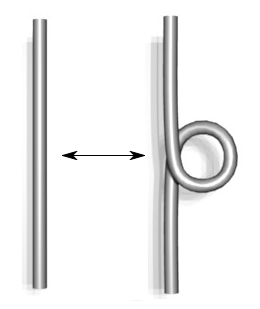
\includegraphics[scale=0.5]{Reidemeister_move_1.png}

\caption{Type 1}

\end{figure}

\vspace{2mm}

\begin{figure}[H]

\centering

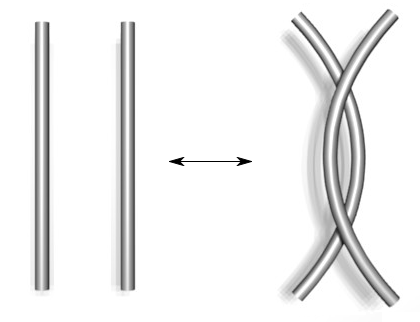
\includegraphics[scale=0.5]{Reidemeister_move_2.png}

\caption{Type 2}

\end{figure}

\pagebreak

\vspace*{-40mm}

\begin{figure}[H]

\centering

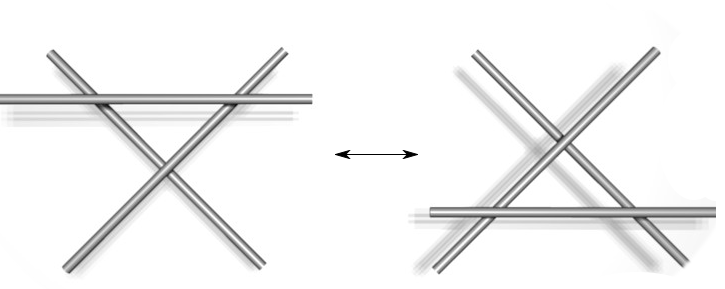
\includegraphics[scale=0.5]{Reidemeister_move_3.png}

\caption{Type 3}

\end{figure}

\vspace{2mm}

\begin{tcolorbox}

\begin{theorem}

\textit{If two links are equivalent, then their diagrams, subject to ambient isotopies of the plane, are related by a sequence of Reidemeister moves.}

\end{theorem}

\end{tcolorbox}

\vspace{2mm}

\begin{tcolorbox}

\begin{definition}

\textit{An \textbf{orientation} of a link is a choice of direction to travel around each component of the link. Consider a crossing a regular projection of an oriented link. Stand on the overpass and face in the direction of the orientation. The crossing is \textbf{right-handed} if and only if traffic on the underpass goes from right to left; the crossing is \textbf{left-handed} if and only if traffic on the underpass goes from left to right. In regular projection of an oriented link of two components, assign +1 to right-handed crossings and -1 to left-handed crossings. Add up the numbers assigned to crossings involving both components. One half this sum is the \textbf{linking number} of the two oriented components of the link.}

\end{definition}

\end{tcolorbox}

\subsection*{2.4 Colorings}

\begin{tcolorbox}

\begin{definition}

\textit{The diagram of a knot is \textbf{colorable} if and only if each arc can be assigned one of three colors subject to the two conditions:}

\begin{center}

\begin{enumerate}

\item At least two colors appear

\item At any crossing where two colors appear, all three colors appear

\end{enumerate}

\end{center}

\end{definition}

\end{tcolorbox}

\vspace{2mm}

\begin{tcolorbox}

\begin{theorem}

\textit{The colorability of a knot diagram is an invariant property of the knot type.}

\end{theorem}

\end{tcolorbox}

\pagebreak

\vspace*{-20mm}

\begin{tcolorbox}

\begin{definition}

\textit{Let p be an odd number greater than two. A knot is p-colorable if at every crossing:}

\begin{center}

\begin{enumerate}

\item At least two colors appear

\item you can solve $color1 + color2 \equiv 2x ~ mod ~ (the ~ number ~ of ~ colors ~ used)$, where color1 and color2 are numbers assigned to the arcs of the knot

\end{enumerate}

\end{center}

\end{definition}

\end{tcolorbox}

\vspace{2mm}

\begin{tcolorbox}

\begin{theorem}

\textit{The colorability of a knot diagram is an invariant property of the knot type.}

\end{theorem}

\end{tcolorbox}

\vspace{2mm}

\begin{tcolorbox}

\begin{theorem}

\textit{The representation of a knot diagram on a wheel with p colors is an invariant property of the knot type.}

\end{theorem}

\end{tcolorbox}

\vspace{2mm}

\begin{tcolorbox}

\begin{definition}

\textit{The determinant of a knot is the absolute value of its Alexander Polynominal evaluated at -1 (simply, plug-in -1 for t)}

\end{definition}

\end{tcolorbox}

\vspace{2mm}

\begin{tcolorbox}

\begin{theorem}

\textit{A knot is p-\textbf{colorable} for prime p greater than two if and only if p divides its determinant}

\end{theorem}

\end{tcolorbox}

\subsection*{2.5 The Alexander Polynominal}

\begin{tcolorbox}

\textit{Steps in computing the Alexander Polynominal:}

\begin{center}

\begin{enumerate}

\item Label the crossings $x_{1}, x_{2}, \cdots, x_{n}$

\item Label the arcs $a_{1}, a_{2}, \cdots, a_{n}$

\item Choose an orientation for the knot

\item As you travel around the knot in the chosen orientation, stand on the overpass of each crossing. Label the overstrand with $1-t$, the left-end of the understrand $t$, and the right-end of the understrand -1

\item Create the arc/crossing matrix

\item Compute the determinant of the matrix, which is the Alexander Polynominal

\end{enumerate}

\end{center}

\end{tcolorbox}

\pagebreak

\vspace*{-30mm}

\begin{tcolorbox}

\begin{definition}

\textit{The projection of an oriented knot divides the plane into a number of regions. The \textbf{index} of one of these regions is the net number of times the projection winds counterclockwise around any point in the region.}

\end{definition}

\end{tcolorbox}

\begin{tcolorbox}

\begin{definition}

\textit{The \textbf{index} of a crossing of a knot diagram is the common value of the index of two of the regions near the crossing.}

\end{definition}

\end{tcolorbox}

\begin{tcolorbox}

\begin{theorem}

\textit{The Alexander Polynominal of an oriented knot is an invariant under Reidemeister moves.}

\end{theorem}

\end{tcolorbox}

\subsection*{2.6 Skein Relations}

\begin{tcolorbox}

\textit{Calculating the $\Delta$ polynominal is the same as calculating the Alexander Polynominal}

\end{tcolorbox}

\subsection*{2.7 The Jones Polynominal}

\begin{tcolorbox}

\textbf{Rules for the Bracket Polynominal} \textit{The Kauffman \textbf{Bracket Polynominal} of a regular projection of a link is a polynominal in integer powers of the variable A defined by the following three rules:}

\begin{center}

\begin{enumerate}
%the first rule
\item
  $\left\langle\KPA\right\rangle=1$

%the second rule
\item
  $\left\langle L \cup \KPA\right\rangle=(-A^{2}-A^{-2})\langle L\rangle$

%the third rule
\item
  $\left\langle\KPB\right\rangle=
  A\left\langle\KPC\right\rangle + A^{-1} \left\langle \KPD \right\rangle$

\end{enumerate}

\end{center}

\end{tcolorbox}

\vspace{2mm}

\begin{tcolorbox}

\begin{definition}

\textit{The \textbf{writhe} w(L) of the regular projection L of a link is the number of right-handed crossings minus the number of left-handed crossings.}

\end{definition}

\end{tcolorbox}

\vspace{2mm}

\begin{tcolorbox}

\begin{definition}

\textit{The X(L) polynominal is defined as:}

\begin{center}

$X(L)=(-A)^{-3w(L)} \big \langle L \big \rangle$, where $\big \langle L \big \rangle$ is the bracket polynominal for L and $w(L)$ is the writhe of L

\end{center}

\end{definition}

\end{tcolorbox}

\pagebreak

\vspace*{-30mm}

\begin{tcolorbox}

\textit{Steps in calculating the Jones Polynominal:}

\begin{center}

\begin{enumerate}

\item Calculate the Bracket Polynominal

\item Calculate the $X-polynominal$

\item Substitute $t^{-\frac{1}{4}}$ in for every ``A" in the $X-polynominal$ and simplify

\end{enumerate}

\end{center}

\end{tcolorbox}

\begin{center}

\section*{Chapter 3 Surfaces}

\end{center}

\subsection*{3.1 Definition and Examples}

\begin{tcolorbox}

\begin{definition}

\textit{In a space with a way of measuring distances between points, a \textbf{neighborhood} of a point is a subset that contains all points within some positive distance of the point}

\end{definition}

\end{tcolorbox}

\vspace{2mm}

\begin{tcolorbox}

\begin{definition}

\textit{A \textbf{surface} (or 2 \textbf{-manifold}) is a space that is homeomorphic to a nonempty subset of finite-dimensional Euclidean space and in which every point has a neighborhood homeomorphic to $\mathbb{R}^{2}$. We sometimes also wish to admit \textbf{boundary} points, which have neighborhoods homeomorphic to the half-plane $\{(x,y) \in \mathbb{R}^{2} ~ | ~ y \geq 0\}$}.

\end{definition}

\end{tcolorbox}

\subsection*{3.2 Cut-and-Paste Techniques}

\begin{tcolorbox}

\begin{definition}

\textit{Let S and T be path-connected surfaces Remove the interior of a disk from each surface by cutting along the boundaries of the disks. Glue the remaining surfaces together along the newly formed boundary components. The result surface is the \textbf{connected sum} of S and T. It is denoted S\texttt{\#}T.}

\end{definition}

\end{tcolorbox}

\subsection*{3.3 The Euler Characteristic and Orientability}

\begin{tcolorbox}

\begin{definition}

\textit{A \textbf{triangulation} of a space is a decomposition of the space into a union of disks, arcs, and points. The disks are called \textbf{faces}, the arcs are called \textbf{edges}, and the points are \textbf{vertices} of the triangulation. A face intersects other components of a triangulation only along its boundary; and the boundary of a face consists of three edges and three vertices. An edge intersects other edges and the vertices only at its endpoints; and both endpoints of an edge are vertices.}

\end{definition}

\end{tcolorbox}

\vspace{2mm}

\begin{tcolorbox}

\begin{definition}

\textit{A triangulated space is \textbf{compact} if and only if it consists of a finite number of faces, edges, and vertices.}

\end{definition}

\end{tcolorbox}

\pagebreak

\vspace*{-30mm}

\begin{tcolorbox}

\begin{definition}

\textit{The \textbf{Euler characteristic} of a compact triangulation space S is the number of vertices minus the number of edges plus the number of faces. The Euler characteristic of S is denoted by $\chi(S)$.}

\end{definition}

\end{tcolorbox}

\begin{tcolorbox}

\begin{theorem}

\textit{Every closed, path-connected surface is homeomorphic to exactly one of:}

\begin{center}

\begin{enumerate}

\item A 2-sphere

\item A connected sum of Tori

\item A connected sum of projective planes

\end{enumerate}

\end{center}

\end{theorem}

\end{tcolorbox}

\vspace{2mm}

\begin{tcolorbox}

\begin{sidenote}

\textit{Something is orientable if it is 2-colorable or doesn't have a mobius band}

\end{sidenote}

\end{tcolorbox}

\begin{tcolorbox}

\begin{theorem}

\textit{Suppose $A$ and $B$ are triangulated so that $A \cap B$ is also triangulated. Then, $\chi(A \cup B)=\chi(A)+\chi(B)-\chi(A \cap B)$}.

\end{theorem}

\end{tcolorbox}

\vspace{2mm}

\begin{tcolorbox}

\begin{theorem}

\textit{The surface formed by taking the connected sum of g tori and cutting out disks to leave b boundary components has Euler characteristic 2-2g-b. The surface formed by taking the connected sum of n projective plane and cutting out disks to leave b boundary components has Euler characteristic 2-n-b}.

\end{theorem}

\end{tcolorbox}

\vspace{2mm}

\begin{tcolorbox}

\begin{definition}

\textit{An \textbf{orientation} of a polygonal face of a triangulated surface is the choice of one of the two possible orientations of the boundary curve of the face. A surface is \textbf{orientable} if and only if it is possible to choose orientations of all the faces of a triangulation of the surface so that whenever two faces share a common edge, the orientation of the faces induce opposite orientations on the edge.}

\end{definition}

\end{tcolorbox}

\vspace{2mm}

\begin{tcolorbox}

\begin{definition}

\textit{$\chi(f_{1}\texttt{\#}f_{2})=\chi(f_{1}) + \chi(f_{2}) - 2$}

\end{definition}

\end{tcolorbox}

\vspace{2mm}

\begin{tcolorbox}

\begin{definition}

\textit{With the word you come up with for the surface, if every letter does not have an inverse, the surface is not orientable. If every letter does have an inverse, it is orientable}

\end{definition}

\end{tcolorbox}

\vspace{2mm}

\begin{tcolorbox}

\begin{definition}

\textit{Just concatenate the two individual words of each surface to get a word for the connected sum of the two surfaces}

\end{definition}

\end{tcolorbox}

\pagebreak

\vspace*{-30mm}

\begin{tcolorbox}

\begin{sidenote}

\textit{The table below helps you figure out what surface is being asked for based on \textbf{Orientability} and the \textbf{Euler characterisitic}}

\vspace{2mm}

\begin{tabular}{||c c c||}

\hline

\textit{$\chi$} & \textit{$Oreintable$} & \textit{$Non-orientable$} \\ [0.5ex]

\hline\hline

2 & Sphere & \\ 

\hline

1 & & P \\

\hline

0 & T & P \texttt{\#} P \\

\hline

-1 &  & P \texttt{\#} P \texttt{\#} P \\

\hline

-2 & T \texttt{\#} T & P \texttt{\#} P \texttt{\#} P \texttt{\#} P  \\

\hline

-3 & & P \texttt{\#} P \texttt{\#} P \texttt{\#} P \texttt{\#} P  \\

\hline

-4 & T \texttt{\#} T \texttt{\#} T & P \texttt{\#} P \texttt{\#} P \texttt{\#} P \texttt{\#} P \texttt{\# P}  \\ [1ex]

\hline

\end{tabular}

\end{sidenote}

\end{tcolorbox}

\end{document}